\documentclass[a4paper,11pt]{article}

\usepackage[margin=2.4cm]{geometry}
\usepackage{amsmath,amssymb,bm}
\usepackage{booktabs}
\usepackage{tikz}
\usepackage{graphicx}
\graphicspath{{figs/}}
\usepackage[dvipsnames]{xcolor}
\usepackage{enumitem}
\usepackage[colorlinks=true,linkcolor=RoyalBlue,citecolor=ForestGreen,urlcolor=RoyalBlue]{hyperref}

%%%%%%%%%%%%%%
%% Notation %%
%%%%%%%%%%%%%%

\newcommand{\vx}{\bm{x}}
\newcommand{\vsv}{\bm{s}}
\newcommand{\vq}{\bm{q}}
\newcommand{\vk}{\bm{k}}
\newcommand{\vp}{\bm{p}}
\newcommand{\vu}{\bm{u}}
\newcommand{\vPsi}{\bm{\Psi}}
\newcommand{\nhat}{\hat{\bm{z}}}
\newcommand{\khat}{\hat{\bm{k}}}
\def\cH{\mathcal{H}}
\def\Plin{P_{\rm L}}
\def\knl{k_{\rm NL}}
\newcommand{\dd}{\mathrm{d}}
\def\dirac{\delta_{\rm D}}
\def\lcdm{$\Lambda$CDM}
\def\Om{\Omega_m}
\def\G{\mathcal{G}}
\numberwithin{equation}{section}

% Short insightful asides
\newenvironment{remark}
  {\par\medskip\noindent\begingroup\small\color{ForestGreen!60!black}\textbf{Comment.}\ }
  {\endgroup\par\medskip}

% Exercises
\newcounter{exercise}[section]
\renewcommand{\theexercise}{\thesection.\arabic{exercise}}
\newenvironment{exercise}
  {\par\medskip\noindent\refstepcounter{exercise}\textbf{Exercise \theexercise.}\ \itshape}
  {\par\medskip}

\title{From Primordial Fluctuations to the Cosmic Web\\[2mm]
\large Lecture notes, two lectures of 90 minutes each,
with two hands-on sessions}
\author{Nhat-Minh Nguyen}
\date{\today\ (draft)}

\begin{document}
\maketitle

\noindent\textbf{Conventions.} Conformal time $\tau$, defined by $\dd t = a\,\dd\tau$, so that $\tau = \int\dd t/a$ --- an integral, not $t/a$; comoving coordinates $\vx$; $\cH \equiv \dd\ln a/\dd\tau = aH$; overdots denote $\partial/\partial\tau$. The comoving background 3-metric is flat, and spatial indices are raised and lowered with $\delta_{ij}$ --- so a repeated pair is summed regardless of placement, and $\partial_k\Phi\,\partial_k\Phi$ means $\sum_k(\partial_k\Phi)^2$. (Under the general-relativistic convention one would move them with $g_{ij}$ instead, which would fold the factor $a^2(1-2\phi)$ into every contraction.) Fourier transforms follow
\begin{equation*}
\delta(\vk) = \int \dd^3x\, e^{-i\vk\cdot\vx}\,\delta(\vx),
\qquad
\delta(\vx) = \int_{\vk} e^{i\vk\cdot\vx}\,\delta(\vk),
\qquad
\int_{\vk} \equiv \int\!\frac{\dd^3k}{(2\pi)^3},
\end{equation*}
so that $\langle\delta(\vk)\delta(\vk')\rangle = (2\pi)^3\dirac(\vk+\vk')P(k)$. A primed correlator, $\langle\cdots\rangle'$, strips the factor $(2\pi)^3\dirac$. Beware: the review~\cite{Bernardeau2002} places the $(2\pi)^{-3}$ on $\dd^3x$ instead, so its power spectra differ by factors of $(2\pi)^3$.

\medskip
\noindent\textbf{Notation.} One table to refer back to; each entry is defined where it first appears.

\begin{center}
\small
\begin{tabular}{@{}ll@{\hspace{2em}}ll@{}}
\toprule
$\tau,\ a,\ \cH$ & conformal time, scale factor, $\cH = \dd\ln a/\dd\tau = aH$; $\dot{} = \partial_\tau$
  & $\vPsi,\ J$ & Lagrangian displacement, Jacobian of $\vq\mapsto\vx$ \\
$\delta,\ \theta$ & density contrast, $\theta = \nabla\cdot\vu$
  & $D_2,\ f_2$ & second-order Lagrangian growth ($D_2<0$), its rate \\
$\Plin(k)$ & linear matter power spectrum
  & $\lambda_1,\lambda_2,\lambda_3$ & eigenvalues of the deformation tensor \\
$D_+,\ f$ & linear growth factor and rate
  & & \\
\bottomrule
\end{tabular}
\end{center}

\tableofcontents

%=====================================================================
\section*{Lecture 1: Linear evolution, the matter power spectrum, and the Zel'dovich picture}
\addcontentsline{toc}{section}{Lecture 1: Linear evolution, the matter power spectrum, and the Zel'dovich picture}
\setcounter{section}{1}
\setcounter{subsection}{0}
\setcounter{equation}{0}
\setcounter{exercise}{0}

\noindent\textbf{Plan (65 min at the board, 25 for questions).} From the SVT decomposition to the linearized Newtonian equations (0--10) $\rightarrow$ the pressureless fluid, the single-stream closure, and linear growth (10--22) $\rightarrow$ Gaussian random fields and what a power spectrum is (22--32) $\rightarrow$ the transfer function and the linear matter power spectrum (32--40) $\rightarrow$ the displacement map, the Zel'dovich approximation, and shell crossing (40--55) $\rightarrow$ 2LPT and why initial conditions need it (55--65). \emph{Read, not lectured:} the geodesic derivation (Exercise~\ref{ex:geodesic}) and the Vlasov hierarchy --- state the single-stream closure and move on. [Timings and split to be rewritten in step 2: this block still describes the three-lecture version.] Sources:~\cite{MaBertschinger1995,Bernardeau2002}, \cite[Apps.~A and E]{Jeong2010}.

\medskip
\noindent\textbf{The setting.} Fixed for the whole course: a spatially flat
Friedmann--Lema\^itre--Robertson--Walker (FLRW) universe --- homogeneous,
isotropic and expanding --- with everything of interest a small departure from
it. The unperturbed metric is
\begin{equation*}
\dd s^2 = a^2(\tau)\left[-\dd\tau^2 + \delta_{ij}\,\dd x^i\dd x^j\right],
\end{equation*}
written in comoving coordinates $\vx$, which ride along with the expansion: a
galaxy at rest keeps the same $\vx$ while its physical separation from us,
$a\vx$, grows. Conformal time is used throughout because of the form this takes:
with $\dd\tau$ and $\dd\vx$ appearing symmetrically, radial light rays obey
$\dd x = \pm\dd\tau$, so light travels at unit comoving speed and an interval of
conformal time \emph{is} a comoving distance. That is what will make the horizon
a clean notion in Section~\ref{sec:bridge}. Structure is what happens when this is not quite true. The metric
picks up small perturbations, and the matter density departs from its mean by
\begin{equation*}
\delta(\vx,\tau) \equiv \frac{\rho(\vx,\tau) - \bar\rho(\tau)}{\bar\rho(\tau)} ,
\end{equation*}
with $|\delta|\ll1$ early on and of order unity by the time there are galaxies to
count. How $\delta$ gets from one to the other is the whole course.

\medskip
\noindent\textbf{Two ways to hold the same field.} We move between them
constantly, so it is worth saying once that they carry identical information.
In \emph{position space}, $\delta(\vx)$ is a lumpy field filling the universe;
this is where physical intuition lives, and where the displacements and
collapsing sheets later in this lecture are easiest to picture. In
\emph{Fourier space}, $\delta(\vk)$ is the amplitude of one plane wave of
comoving wavelength $\lambda = 2\pi/k$ --- so large $k$ means small scales, and
$k = 0.1\,h\,{\rm Mpc}^{-1}$ means $\lambda \simeq 63\,h^{-1}{\rm Mpc}$, a few
cluster diameters. This is where the dynamics and the statistics live. The
transform convention is in the front matter; nothing below depends on which
picture you find more natural, only on being fluent in both.
Figure~\ref{fig:fourier} is the same statement drawn.

\begin{figure}[t]
\centering
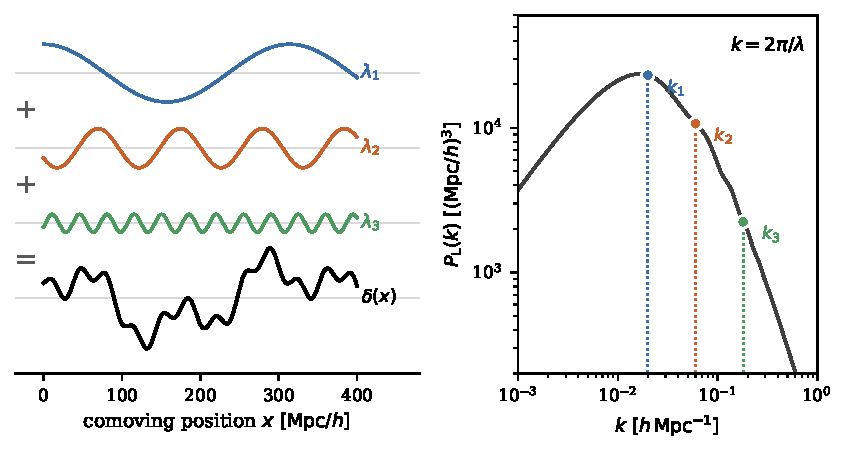
\includegraphics[width=0.96\textwidth]{fourier_decomposition.pdf}
\caption{The same field, held two ways. \emph{Left:} three plane waves of
comoving wavelength $\lambda = 2\pi/k$, added into a lumpy density field
$\delta(x)$. This is a one-dimensional slice for legibility; the real field is
three-dimensional and each mode carries a direction $\khat$ as well as a
wavelength. \emph{Right:} where those same three modes sit on the linear power
spectrum, which is nothing more exotic than amplitude against scale (defined
properly in Section~\ref{sec:stats}, and computed in Section~\ref{sec:linearpk}).
Colours identify the same mode across the two panels.
\newline
One warning, because the picture invites the wrong conclusion. The longest wave
is drawn with the largest amplitude, correctly: a single mode's amplitude goes
as $\sqrt{\Plin(k)}$, and $\Plin$ falls beyond its peak. But that is \emph{not}
the same as large scales dominating the lumpiness. Short-wavelength modes are
far more numerous, and the fluctuation power per logarithmic interval,
$\Delta^2(k) = k^3\Plin(k)/2\pi^2$, rises steeply across these three modes ---
$0.009$, $0.12$, $0.66$. Small scales carry more, which is why nonlinearity
reaches them first, and why almost everything difficult in this course happens
at large $k$.}
\label{fig:fourier}
\end{figure}

\subsection{Why Newtonian dynamics, and which \texorpdfstring{$\delta$}{delta}}
\label{sec:bridge}

Newtonian gravity is two statements: particles fall down a potential,
$\ddot\vx = -\nabla\Phi$, and the potential is sourced by density,
$\nabla^2\Phi = 4\pi G\rho$. Recovering each from general relativity takes a
\emph{different} limit, and it is worth seeing which is which.

\paragraph{Why Fourier, for the dynamics.} Of the two pictures, the linear
problem wants the second one, and not merely for convenience. The linearized
equations are linear with coefficients that do not depend on position --- the
background is homogeneous --- so a plane wave stays a plane wave, and each
$\delta(\vk)$ evolves independently of every other. One partial differential
equation in three dimensions becomes one ordinary differential equation per
$\vk$. That is what makes linear theory solvable at all, and losing it is what
makes everything afterwards hard: nonlinear terms couple modes together, and
organising that coupling is what perturbation theory beyond linear order is for, and it is the subject of the companion notes \cite{EFTnotes}.

One point about the label. Because $\vk$ is comoving it is fixed once and for
all; it does not change as the universe expands, and what grows is the physical
wavelength $a\lambda$. Nothing in the next paragraph happens because a mode
changes. It happens because the horizon does.

\paragraph{The horizon.} Write $\cH \equiv \dd\ln a/\dd\tau = aH$, the expansion
rate in conformal time --- not the Hubble parameter $H \equiv \dd\ln a/\dd t$.
(Overdots in these notes are $\partial/\partial\tau$ throughout, so $\dot a/a$ is
$\cH$, not $H$. It is also why the growth equation \eqref{eq:growth} below
carries $\cH\dot D$ where its cosmic-time form carries $2H\,\dd D/\dd t$.)
Because $\cH$ is a
\emph{logarithmic} rate --- the fractional growth of $a$ per unit conformal time
--- its definition rearranges to $\Delta\tau = \Delta\ln a/\cH$. One e-fold means
$\Delta\ln a = 1$, so $1/\cH$ is the conformal time in which $a$ grows by a
factor $e$: exactly if $\cH$ held still, and to a factor of order one otherwise
($1.7/\cH$ in radiation domination, $1.3/\cH$ in matter domination; exactly
$1/\cH$ only in de Sitter, where $\cH$ really is constant). Since light moves at
unit comoving speed in conformal time, that same number is the comoving distance
light covers while it happens: the comoving Hubble radius. A time interval and a
length, one number. Loosely, ``the horizon''; strictly it is the Hubble radius, not
the particle horizon $\int\!\dd t/a = \tau$, though in power-law eras the two
agree to a factor of order one ($1/\cH = \tau$ in radiation domination,
$\tau/2$ in matter domination). A mode of comoving wavenumber $k$ is
\emph{sub-horizon} when $k \gg \cH$, meaning its wavelength is short compared
with $1/\cH$, and \emph{super-horizon} when $k \ll \cH$. Inside the horizon a
signal crosses the perturbation many times per expansion time, so gravity and
pressure act coherently across it and local physics is meaningful. Outside,
nothing propagates across the mode at all. You have met the comoving Hubble radius before, running the other way. During
inflation it \emph{shrinks}, which is how modes exit and how their fluctuations
are frozen in as initial conditions. Afterwards it grows, through radiation and
matter domination alike, so a given $k$ starts super-horizon and \emph{enters}
the horizon when $k = \cH$. That is the decisive event in the life of a mode:
what happens to it depends almost entirely on when it entered, which is what the
transfer function of Section~\ref{sec:linearpk} records.

\paragraph{The metric.} Fix the gauge completely with the conformal Newtonian
(longitudinal) form \cite{MaBertschinger1995},
\begin{equation}
\dd s^2 = a^2(\tau)\left[-(1+2\psi)\,\dd\tau^2 + (1-2\phi)\,\delta_{ij}\,\dd x^i\dd x^j\right] .
\label{eq:newtonian_gauge}
\end{equation}
Here $\psi$ perturbs $g_{00}$ and $\phi$ perturbs the spatial metric. Keep them
apart for the moment: the two limits below use different ones, which is the
point.

\paragraph{First limit: slow motion gives the force law.} For a particle with
$v \ll 1$, the geodesic equation in the metric \eqref{eq:newtonian_gauge}
reduces to
\begin{equation}
\ddot\vx + \cH\,\dot\vx = -\nabla\psi
\label{eq:newtonian_eom}
\end{equation}
(Exercise~\ref{ex:geodesic}), which is Newton's second law in comoving
coordinates, with $\cH\dot\vx$ the drag from expansion. So $\psi$, the
perturbation to $g_{00}$, \emph{is} the Newtonian potential. Note what was
required: only that the matter moves slowly. Nothing about $k$.

\paragraph{Second limit: sub-horizon gives the field equation.} The horizon
enters through the field equation instead. One linearized Einstein equation is
the energy constraint \cite[Eq.~(23a)]{MaBertschinger1995},
\begin{equation}
\underbrace{k^2\phi}_{\text{sub-horizon}} +
\underbrace{3\cH\big(\dot\phi + \cH\psi\big)}_{\text{super-horizon}}
= -4\pi G a^2\bar\rho\,\delta .
\label{eq:energy_constraint}
\end{equation}
For $k \gg \cH$ the second group is smaller than the first by $(\cH/k)^2$ and
drops, leaving $-k^2\phi = 4\pi Ga^2\bar\rho\,\delta$: the Poisson equation.
Super-horizon it is the other way round, and there is no Poisson equation to be
had.

Two limits, two jobs --- and two \emph{different} potentials. Slow motion gives
the force law, sourced by $\psi$; sub-horizon gives the field equation, obeyed
by $\phi$. Newtonian gravity has only one potential, so the last thing needed is
that these coincide. They do whenever the total anisotropic stress vanishes
\cite[Eq.~(23d)]{MaBertschinger1995}, which holds for CDM and baryons in the
matter era; free-streaming neutrinos spoil it at the $15\%$ level during
radiation domination, but that contribution fades as matter comes to dominate.
Setting $\phi = \psi \equiv \Phi$ then closes the system --- and two of its three
equations are already in hand. Write the velocity field as $\vu = \dot\vx$ and
its divergence as $\theta \equiv \nabla\cdot\vu$. At linear order the derivative
along a trajectory reduces to $\partial_\tau$, since the advective piece
$\vu\cdot\nabla$ acting on a first-order quantity is second order, so the force
law \eqref{eq:newtonian_eom} is already a field equation; taking its divergence
and substituting the Poisson equation gives the second line below. The third
line \emph{is} the sub-horizon limit of \eqref{eq:energy_constraint}. Only the
first is genuinely new, and it is bookkeeping rather than dynamics --- linearized
mass conservation, whose relativistic dilation term $3\dot\phi$ drops by the same
$(\cH/k)^2$:
\begin{equation}
\dot\delta = -\theta,
\qquad
\dot\theta = -\cH\,\theta - \frac{3}{2}\Om(\tau)\cH^2\delta,
\qquad
\nabla^2\Phi = \frac{3}{2}\Om(\tau)\cH^2\delta ,
\label{eq:newtonian_linear}
\end{equation}
with $\vu \equiv \dd\vx/\dd\tau$,
$\theta \equiv \nabla\cdot\vu$, and $4\pi Ga^2\bar\rho = \tfrac32\Om\cH^2$.

\paragraph{Which \texorpdfstring{$\delta$}{delta}.} One more thing is settled by
$k \gg \cH$, and it is the one students are usually not told. Relativistically
$\delta$ is not a physical quantity: it depends on how spacetime is sliced. The
same mode grows as $(k\tau)^2$ in synchronous gauge and sits frozen in the
Newtonian gauge until horizon entry \cite[\S 7]{MaBertschinger1995} --- which is
why ``do perturbations grow outside the horizon?'' has no gauge-independent
answer. Sub-horizon that ambiguity is suppressed by the same $(\cH/k)^2$, and
$\delta$ becomes something unambiguous to compute, correlate and measure. Every
power spectrum in these lectures stands on that.

\paragraph{Why the metric stays linear.} One consequence of the Poisson equation
is worth drawing out now, because everything after this lecture depends on it.
Inverting $-k^2\Phi = 4\pi Ga^2\bar\rho\,\delta$ gives
\begin{equation}
|\Phi| \sim \frac{3}{2}\,\Om\left(\frac{\cH}{k}\right)^{\!2}\delta ,
\label{eq:phi_small}
\end{equation}
so the potential is the density contrast suppressed by two powers of $\cH/k$ ---
the same factor that licensed the Newtonian limit. At
$k = 0.1\,h\,{\rm Mpc}^{-1}$ that suppression is about $10^{-5}$, so even a patch
with $\delta \sim 100$ carries $|\Phi| \sim 5\times10^{-4}$. Gravity stays weak
precisely where clustering becomes strong.

This is the licence for the rest of the course. We will let $\delta$ grow to
order unity and beyond, and resum it to all orders through loops and
displacements, while never going past linear order in the metric. Those two
statements sound contradictory and are not: $\Phi$ and $\delta$ are separated by
$(\cH/k)^2$, and it is $\delta$ alone that becomes large.

\begin{remark}
The window, then. It closes below at $k\sim\cH$, in practice
$k \sim 10^{-3}\,h\,{\rm Mpc}^{-1}$, where relativistic corrections and the gauge
question both return \cite{Huterer2023}. It does \emph{not} close from pressure:
the post-recombination Jeans scale corresponds to a mass of order
$10^5\,M_\odot$, far below anything here, so cold and pressureless is safe. What
closes it from above is nonlinearity, and two distinct things fail at different
points. The \emph{linearization} goes first, near
$k\sim0.1\,h\,{\rm Mpc}^{-1}$; \eqref{eq:newtonian_linear} is the linearized form
of equations that are themselves nonlinear, and recovering those is the next
section's business. The \emph{Newtonian description} survives further but not
indefinitely, and where it fails is what Lecture~2 is about.
\end{remark}

\subsection{The Vlasov equation and the pressureless fluid}
\label{sec:vlasov}

We now set up the nonlinear problem in the Newtonian regime, following \cite[\S 2]{Bernardeau2002}. Particles obey \eqref{eq:newtonian_eom}, with $\Phi$ the peculiar potential of \eqref{eq:newtonian_linear}. Collisionless matter is then described by its phase-space density $f(\vx,\vp,\tau)$, with $\vp = am\vu$; phase-space conservation gives the Vlasov equation,
\begin{equation}
\frac{\partial f}{\partial\tau} + \frac{\vp}{ma}\cdot\nabla f - am\,\nabla\Phi\cdot\frac{\partial f}{\partial\vp} = 0 .
\label{eq:vlasov}
\end{equation}
Taking velocity moments produces a hierarchy: the zeroth moment gives continuity, the first gives the Euler equation, and each couples to the next through the velocity-dispersion tensor $\sigma_{ij} \equiv \langle u_iu_j\rangle_p - \langle u_i\rangle_p\langle u_j\rangle_p$, where $\langle\cdot\rangle_p$ denotes the momentum average over $f$ at fixed $(\vx,\tau)$ (not the ensemble average of Section~\ref{sec:stats}):
\begin{align}
\dot\delta + \nabla\cdot\left[(1+\delta)\,\vu\right] &= 0 ,
\label{eq:continuity}\\
\dot{\vu} + \cH\,\vu + (\vu\cdot\nabla)\,\vu &= -\nabla\Phi - \frac{1}{\rho}\,\nabla_j\!\left(\rho\,\sigma_{ij}\right).
\label{eq:euler}
\end{align}
Cold matter starts cold: before orbits cross, each position hosts a single stream and $\sigma_{ij} = 0$. This \emph{single-stream closure} truncates the hierarchy into a pressureless perfect fluid. It is a closure rather than a controlled approximation: exact until shell crossing, and completely wrong after. Where it fails is where the effective theory of Lecture~2 will operate.

Within the closure, vorticity $\bm{w} = \nabla\times\vu$ obeys a homogeneous equation: it decays as $1/a$ at linear order and stays zero if it starts zero. The velocity field is then fully specified by its divergence $\theta = \nabla\cdot\vu$.

Linearizing \eqref{eq:continuity}--\eqref{eq:euler} recovers \eqref{eq:newtonian_linear}, which combine into
\begin{equation}
\ddot D + \cH\,\dot D - \frac{3}{2}\Om(\tau)\,\cH^2 D = 0 .
\label{eq:growth}
\end{equation}
The growing solution $D_+(\tau)$ defines linear growth, $\delta^{(1)}(\vx,\tau) = D_+(\tau)\,\delta_0(\vx)$; in Einstein--de Sitter (EdS, $\Om = 1$) $D_+ = a$ and the decaying mode is $a^{-3/2}$. The velocity follows from continuity, and introduces the growth rate $f$ (not to be confused with the phase-space density of \eqref{eq:vlasov}, the one unfortunate collision in the standard notation),
\begin{equation}
\theta^{(1)} = -\cH f\,\delta^{(1)},
\qquad
f \equiv \frac{\dd\ln D_+}{\dd\ln a}
\simeq \Om^{5/9}(\tau) \quad\text{(flat \lcdm)} ,
\label{eq:growth_rate}
\end{equation}
with $f = 1$ in EdS. The often-quoted exponent $0.55$~\cite{Linder2005} agrees with $5/9$ at the sub-percent level over viable cosmologies. The growth rate will return as the central quantity of redshift-space distortions in Lecture~3.

\subsection{Gaussian random fields and the power spectrum}
\label{sec:stats}

Inflation delivers, to very good approximation, Gaussian initial conditions: the linear field $\delta^{(1)}(\vk)$ is a Gaussian random field, meaning that any finite set of its Fourier modes is jointly Gaussian with zero mean. Such a field is characterized completely by its power spectrum,
\begin{equation}
\langle \delta^{(1)}(\vk)\,\delta^{(1)}(\vk')\rangle = (2\pi)^3\dirac(\vk+\vk')\,\Plin(k) ,
\label{eq:plin_def}
\end{equation}
where two distinct assumptions are at work. Statistical \emph{homogeneity} --- invariance under translations --- is what forces the delta function, so that modes whose wavevectors do not sum to zero are uncorrelated. Statistical \emph{isotropy} is a separate statement, invariance under rotations, and it is what makes $\Plin$ a function of the magnitude $k=|\vk|$ alone rather than of the vector $\vk$. Note the one pair that is exempt: $\vk' = -\vk$, where the delta function fires. Since the field is real, $\delta(-\vk) = \delta(\vk)^*$, so that case is $\langle|\delta(\vk)|^2\rangle$ --- a variance, and necessarily non-negative. It is not a counterexample to ``uncorrelated'' but the definition of $\Plin$ itself.

That a Gaussian field is specified completely by $\Plin$ is a practical statement as much as a formal one. To \emph{generate} a realization you draw each Fourier mode independently, with variance $\Plin(k)$ and a random phase, and transform back. That is the first step of any initial-conditions code, and the first step of the hands-on session.

\subsection{The linear matter power spectrum}
\label{sec:linearpk}

The linear evolution across horizon entry and the radiation--matter transition is what a Boltzmann code integrates. Its output is summarized by the transfer function: modes with $k > k_{\rm eq}$ entered the horizon during radiation domination, when CDM perturbations could barely grow (the M\'esz\'aros effect), so they carry a suppression that larger-scale modes escape. Modes entering after equality avoid it and, once sub-horizon in matter domination, grow approximately as $a$. (Note the care needed after the Comment in Section~\ref{sec:bridge}: a mode that is still super-horizon is \emph{not} growing as $a$ in the Newtonian gauge.) The value $k_{\rm eq} \simeq 0.015\,h\,{\rm Mpc}^{-1}$ is fiducial --- it depends on $\Om h^2$ and on the radiation density. The processed spectrum, including the baryon acoustic oscillation (BAO) wiggles imprinted by the pre-recombination photon--baryon fluid, is what fixes the shape of the $\Plin(k,z)$ defined in \eqref{eq:plin_def}. Everything in these lectures takes $\Plin$ as the input.

\subsection{The Lagrangian picture and the Zel'dovich approximation}
\label{sec:lpt}

How does gravitational collapse actually proceed? A slightly overdense region decelerates the matter around it; particles drift toward it, overshoot, and eventually orbit. The natural variable for this story is not the density at a fixed point but the trajectory of each mass element. Label each fluid element by its initial comoving position $\vq$ and track its displacement,
\begin{equation}
\vx(\vq,\tau) = \vq + \vPsi(\vq,\tau),
\qquad \vPsi(\vq,0)=0 .
\label{eq:displacement}
\end{equation}
This is Lagrangian perturbation theory (LPT). The particle equation of motion \eqref{eq:newtonian_eom} governs $\vPsi$; taking its divergence and using the Poisson equation,
\begin{equation}
\nabla_x\cdot\left[\ddot\vPsi + \cH\,\dot\vPsi\right]
= -\,\frac{3}{2}\,\Om(\tau)\,\cH^2\,\delta\big(\vx(\vq,\tau)\big) .
\label{eq:lpt_master}
\end{equation}
The density needs no equation of its own. Mass conservation, $\bar\rho\,\dd^3q = \rho(\vx)\,\dd^3x$, fixes it algebraically from the volume distortion of the map:
\begin{equation}
1 + \delta(\vx,\tau) = \frac{1}{J(\vq,\tau)},
\qquad
J = \det\left(\delta_{ij} + \Psi_{i,j}\right),
\qquad
\Psi_{i,j} \equiv \frac{\partial\Psi_i}{\partial q_j} .
\label{eq:jacobian}
\end{equation}
A volume element that shrinks ($J<1$) is overdense; one that expands is underdense. Because the determinant is nonlinear in $\vPsi$, a displacement of first order generates density perturbations at all orders: low-order LPT resums an infinite subset of Eulerian nonlinearities, the ones associated with moving matter around. The subset is real but restricted --- the Jacobian generates every power of the linear displacement, not every dynamical nonlinearity --- so more orders in density does not mean more dynamical accuracy at all scales.

At first order, \eqref{eq:lpt_master} with $\delta = -\nabla_q\cdot\vPsi^{(1)}$ (from \eqref{eq:jacobian}) says that the divergence of the displacement obeys the linear growth equation \eqref{eq:growth}. Since the flow is irrotational, $\vPsi^{(1)} = -\nabla_q\varphi^{(1)}$ for a Lagrangian potential $\varphi^{(1)}$, and matching to the Eulerian linear density gives
\begin{equation}
\nabla_q\cdot\vPsi^{(1)}(\vq,\tau) = -\,\delta^{(1)}(\vq,\tau)
\qquad\Longleftrightarrow\qquad
\vPsi^{(1)}(\vk,\tau) = \frac{i\vk}{k^2}\,\delta^{(1)}(\vk,\tau) .
\label{eq:za_displacement}
\end{equation}
The \emph{Zel'dovich approximation} (ZA) \cite{Zeldovich1970} takes this linear displacement seriously beyond linear order in the density: move particles on straight lines (in comoving coordinates) and read the density off the Jacobian. Since $\Psi^{(1)}_{i,j}$ is symmetric it can be diagonalized at each $\vq$, with eigenvalues written $-D_+\lambda_1, -D_+\lambda_2, -D_+\lambda_3$, so
\begin{equation}
\delta_{\rm ZA}(\vx,\tau)
= \frac{1}{\left(1-D_+\lambda_1\right)\left(1-D_+\lambda_2\right)\left(1-D_+\lambda_3\right)} - 1 .
\label{eq:za_density}
\end{equation}
Here is the physical picture of structure formation, sketched in Fig.~\ref{fig:collapse}. At each point the initial conditions define three principal axes with collapse strengths $\lambda_1 > \lambda_2 > \lambda_3$. They are generically unequal for a simple statistical reason: the eigenvalues of a random symmetric matrix are almost never degenerate, so perfectly spherical collapse essentially never happens. Collapse happens first along the $\lambda_1$ axis, when $D_+\lambda_1 \to 1$: matter flattens into a sheet, a Zel'dovich \emph{pancake}, and the density formally diverges. That moment, $J \to 0$, is \emph{shell crossing}. Particle trajectories intersect, the map $\vq\mapsto\vx$ stops being invertible, several streams with different velocities coexist at the same point, and both the single-stream description of Section~\ref{sec:vlasov} and the Zel'dovich solution itself stop being valid.

It is worth being clear about what the rest of Fig.~\ref{fig:collapse} is, then. Formally the second factor in \eqref{eq:za_density} vanishes later wherever $\lambda_2>0$, and the third later still wherever $\lambda_3>0$; the sequence sheet $\rightarrow$ filament $\rightarrow$ knot is that ordering of eigenvalue crossings, and nothing more. As a guide to the \emph{morphology} of the cosmic web it is an excellent one, and it is why the ZA predicts the skeleton of that web from the second derivatives of the initial potential alone. As dynamics past the first caustic it is an extrapolation: a Zel'dovich knot is not a halo, and the approximation says nothing about binding, virialization, or the stable orbiting configuration that collapsed matter actually settles into. Getting through shell crossing needs adhesion models, phase-space methods, or $N$-body simulation.

\begin{figure}[t]
\centering
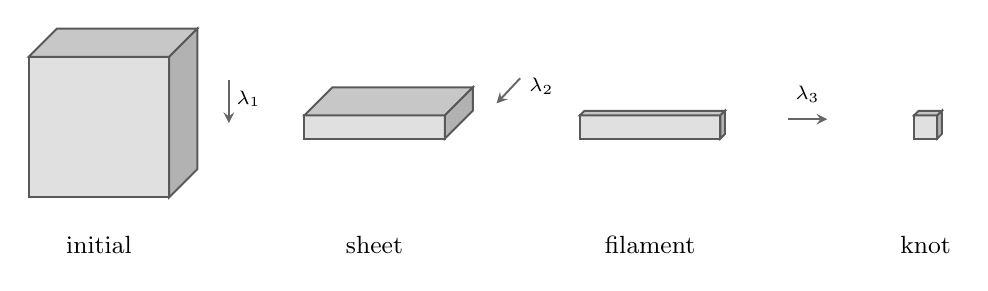
\begin{tikzpicture}[line width=0.7pt, scale=1.0]
% each panel: a box with axis labels, drawn in oblique projection so all three
% axes are visible and each successive collapse is a visible flattening
\newcommand{\panel}[5]{% #1 x-shift, #2 label, #3 sx, #4 sy, #5 sz(depth)
  \begin{scope}[xshift=#1 cm]
    \pgfmathsetmacro{\ax}{1.05*#3}
    \pgfmathsetmacro{\ay}{1.05*#4}
    \pgfmathsetmacro{\dz}{0.42*#5}
    \filldraw[fill=black!12, draw=black!65]
      (-\ax,-\ay) -- (\ax,-\ay) -- (\ax,\ay) -- (-\ax,\ay) -- cycle;
    \filldraw[fill=black!22, draw=black!65]
      (-\ax,\ay) -- (\ax,\ay) -- (\ax+\dz,\ay+\dz) -- (-\ax+\dz,\ay+\dz) -- cycle;
    \filldraw[fill=black!30, draw=black!65]
      (\ax,-\ay) -- (\ax+\dz,-\ay+\dz) -- (\ax+\dz,\ay+\dz) -- (\ax,\ay) -- cycle;
    \node at (0,-1.5) {\small #2};
  \end{scope}}
\panel{0}{initial}{0.85}{0.85}{0.85}
\panel{3.5}{sheet}{0.85}{0.14}{0.85}
\panel{7.0}{filament}{0.85}{0.14}{0.14}
\panel{10.5}{knot}{0.14}{0.14}{0.14}
% collapse arrows, each drawn along the axis that collapses at that step
\draw[->,>=stealth,black!60] (1.65,0.60) -- (1.65,0.05);        % vertical
\node at (1.90,0.36) {\scriptsize $\lambda_1$};
\draw[->,>=stealth,black!60] (5.35,0.62) -- (5.05,0.30);        % into the page
\node at (5.62,0.52) {\scriptsize $\lambda_2$};
\draw[->,>=stealth,black!60] (8.75,0.10) -- (9.25,0.10);        % horizontal
\node at (9.00,0.42) {\scriptsize $\lambda_3$};
\end{tikzpicture}
\caption{The Zel'dovich eigenvalue sequence, drawn in oblique projection so that all three axes are visible. A patch flattens along its principal axes in order of decreasing $\lambda_i$, each stage occurring when the corresponding factor $1-D_+\lambda_i$ in \eqref{eq:za_density} passes through zero: first the vertical axis, giving a sheet, then the depth axis, then the last one --- the second and third only where $\lambda_2$ and $\lambda_3$ are themselves positive, so many patches stop at a sheet. \emph{Only the first crossing is dynamics.} It is a genuine ZA prediction, and it requires a sufficiently positive $\lambda_1$ and enough subsequent growth, so it is not guaranteed at an arbitrary point in a late-time accelerating universe. The second and third stages lie beyond the first caustic, where the approximation has already broken down; read them as the formal eigenvalue ordering, which tracks the morphology of the cosmic web, and not as a description of collapse. The final object is a knot in the deformation map, not a virialized halo.}
\label{fig:collapse}
\end{figure}

\begin{remark}
The ZA is not a degraded linear theory. Its density field \eqref{eq:za_density} contains terms of all orders, and it captures the physics that dominates on quasi-linear scales --- bulk motion --- nonperturbatively. (Exactly, in one dimension before shell crossing, as in Exercise~\ref{ex:1dza}; in three dimensions it is a very good approximation to the displacement, not an exact solution.) This is why the ZA describes the smearing of the BAO feature much better than linear Eulerian theory, why it generates initial conditions for $N$-body simulations, and why its descendants power the infrared resummation of Lecture~3.
\end{remark}

\subsection{Second order: 2LPT and initial conditions}
\label{sec:2lpt}

At second order the displacement responds to the gravitational tide generated at first order. Expanding \eqref{eq:lpt_master} and \eqref{eq:jacobian} to second order, the divergence $\Psi^{(2)}_{i,i}$ obeys the linear-growth operator with a quadratic source \cite[Eqs.~(E.30)--(E.31)]{Jeong2010}; separating variables, the second-order growth factor obeys
\begin{equation}
\ddot D_2 + \cH\dot D_2 - \frac{3}{2}\Om\cH^2 D_2
= -\frac{3}{2}\Om\cH^2 D_+^2 ,
\qquad
D_2(\tau) \simeq -\frac{3}{7}\,D_+^2(\tau)\;\Om^{-1/143},
\label{eq:D2}
\end{equation}
where the fit is accurate to $0.6\%$ for flat \lcdm{} and the EdS limit is $D_2 = -\tfrac37 D_+^2$. (This Lagrangian $D_2$ is a different object from the second-order amplitude of Eulerian perturbation theory \cite{EFTnotes}; the literature uses the same symbol for both.) The spatial source is the second principal invariant of the deformation tensor $\varphi^{(1)}_{,ij}$: writing $\vPsi^{(2)} = \nabla_q\varphi^{(2)}$,
\begin{equation}
\nabla_q^2\varphi^{(2)}
\simeq -\frac{3}{7}\,\Om^{-1/143}
\sum_{i>j}\Big[\varphi^{(1)}_{,ii}\,\varphi^{(1)}_{,jj} - \big(\varphi^{(1)}_{,ij}\big)^2\Big],
\label{eq:2lpt_potential}
\end{equation}
with $\vPsi^{(1)} = -\nabla_q\varphi^{(1)}$ and $\nabla^2_q\varphi^{(1)} = \delta^{(1)}$, both understood as full-time fields with their growth factors included. Do not read \eqref{eq:2lpt_potential} as a purely tidal source: the invariant decomposes into an isotropic piece built from $\delta^2$ and a trace-free tidal piece, and it is nonzero even for a spherical patch, as Exercise~\ref{ex:d2} makes explicit. The full 2LPT map, including velocities, is
\begin{equation}
\vx = \vq - \nabla_q\varphi^{(1)} + \nabla_q\varphi^{(2)},
\qquad
\vu = -\cH f_1 \nabla_q\varphi^{(1)} + \cH f_2\nabla_q\varphi^{(2)},
\qquad
f_2 \simeq 2\,\Om^{6/11} ,
\label{eq:2lpt_map}
\end{equation}
where $f_1 \equiv \dd\ln D_+/\dd\ln a = f$ and, because the convention here has $D_2<0$ so that $\ln D_2$ is undefined,
\begin{equation}
f_2 \equiv \frac{\dd\ln|D_2|}{\dd\ln a} = \frac{\dot D_2}{\cH D_2} .
\label{eq:f2_def}
\end{equation}
The velocity in \eqref{eq:2lpt_map} is unaffected by this: the sign of $D_2$ already sits in $\varphi^{(2)}$. Physically: Zel'dovich streams are straight; the tide bends them. 2LPT is the standard for setting up initial conditions of $N$-body simulations: starting from the ZA alone leaves slowly decaying transients, and 2LPT strongly suppresses them. How large the residual is depends on the starting redshift, the force resolution, and which statistic you look at \cite[App.~E.5]{Jeong2010}.

\begin{remark}
Sign conventions differ across the literature: here $D_2<0$ and the map carries $+\nabla_q\varphi^{(2)}$ \cite[App.~E]{Jeong2010}; other references absorb the minus sign into $D_2$. Check before comparing codes.
\end{remark}

Do the Lagrangian and Eulerian descriptions carry the same information?
Order by order, and before shell crossing, yes --- the companion notes
\cite{EFTnotes} make the correspondence explicit by recovering the Eulerian
kernels from the displacement map.

\begin{exercise}\label{ex:geodesic}
Derive \eqref{eq:newtonian_eom}: write the geodesic equation for a nonrelativistic particle in the metric \eqref{eq:newtonian_gauge}, keep terms to first order in the potentials and to leading order in $u \ll 1$, and use $\phi = \psi = \Phi$. Careful: conformal time is not an affine parameter.
\end{exercise}

\begin{exercise}\label{ex:subhorizon}
\textbf{The other limit.} Exercise~\ref{ex:geodesic} took $v\ll1$ and produced
the force law; this one takes $k\gg\cH$ and produces the field equation.
(i) Reducing \eqref{eq:energy_constraint} to Poisson needs slightly more than
$k\gg\cH$: it needs $\dot\phi$ not to be anomalously large. Assuming
$\dot\phi \lesssim \cH\phi$, which holds for the growing mode, show that the
discarded group is smaller than the retained one by
$\mathcal{O}\big((\cH/k)^2\big)$.
(ii) Put a number on it. Today $\cH_0 = H_0/c \simeq 3.3\times10^{-4}\,h\,{\rm Mpc}^{-1}$.
How large is the neglected term at $k = 0.1\,h\,{\rm Mpc}^{-1}$, and at
$k = 10^{-3}\,h\,{\rm Mpc}^{-1}$? Which of the two lies inside the window quoted
in the Comment above?
(iii) The assumption in (i) can be \emph{removed} rather than justified:
combining the time--time constraint with the time--space one gives an algebraic
equation for $\phi$ carrying no time derivative at all, in which the correction
is manifestly $\mathcal{O}(\cH/k)$ \cite[Ex.~6.7]{DodelsonSchmidt}. Why is
eliminating an assumption preferable to bounding it?
\end{exercise}

\begin{exercise}\label{ex:d2}
Solve \eqref{eq:D2} in EdS ($\cH = 2/\tau$, $\Om=1$, $D_+ = a \propto \tau^2$) and verify $D_2 = -\tfrac37 a^2$.
\end{exercise}

\begin{exercise}\label{ex:1dza}
\textbf{(Optional.)} In one spatial dimension the Zel'dovich approximation is exact until shell crossing. Prove this by showing that the 1D displacement $\Psi^{(1)}$ solves the full nonlinear equation of motion, using the fact that in 1D the force on a sheet depends only on the mass on either side of it. Assume plane-parallel sheets, a subtracted homogeneous background, and boundary conditions (periodic, or a fixed reference point) that determine the constant in $\int\delta\,\dd x$.
\end{exercise}

\appendix
\section*{Appendices}
\addcontentsline{toc}{section}{Appendices}
\setcounter{section}{0}
\renewcommand{\thesection}{\Alph{section}}
\setcounter{equation}{0}
\renewcommand{\theequation}{\thesection.\arabic{equation}}

\noindent A short glossary of words the lectures use without ceremony.

\section{Glossary}
\label{app:glossary}

Words used in the lectures without ceremony, in case any are new.

\begin{center}
\small
\begin{tabular}{@{}p{0.20\textwidth}p{0.76\textwidth}@{}}
\toprule
Boltzmann code & program integrating the linear relativistic equations for all species (\texttt{CAMB}, \texttt{CLASS}); supplies $\Plin$ and growth quantities \\
transfer function & the resulting ratio of a mode's late-time to primordial amplitude, encoding processing through horizon entry and equality \\
M\'esz\'aros effect & the near-freezing of CDM growth for modes inside the horizon during radiation domination \\
$h$ & the Hubble constant in units of $100\,{\rm km\,s^{-1}Mpc^{-1}}$; distances carry $h^{-1}$Mpc so that this choice cancels \\
$N$-body simulation & direct numerical integration of gravitating particles, valid past shell crossing where perturbation theory is not \\
tracer & any observed population standing in for the matter field (galaxies, quasars, halos) \\
\bottomrule
\end{tabular}
\end{center}

\begin{thebibliography}{99}

\bibitem{MaBertschinger1995}
C.-P. Ma and E. Bertschinger,
\emph{Cosmological perturbation theory in the synchronous and conformal Newtonian gauges},
Astrophys. J. \textbf{455} (1995) 7
[\href{https://arxiv.org/abs/astro-ph/9506072}{astro-ph/9506072}].

\bibitem{Bernardeau2002}
F. Bernardeau, S. Colombi, E. Gazta\~naga and R. Scoccimarro,
\emph{Large-scale structure of the universe and cosmological perturbation theory},
Phys. Rept. \textbf{367} (2002) 1
[\href{https://arxiv.org/abs/astro-ph/0112551}{astro-ph/0112551}].

\bibitem{Zeldovich1970}
Y.~B. Zel'dovich,
\emph{Gravitational instability: An approximate theory for large density perturbations},
Astron. Astrophys. \textbf{5} (1970) 84.

\bibitem{EFTnotes}
N.-M. Nguyen,
\emph{Cosmological perturbation theory from matter to galaxies},
companion lecture notes (\texttt{EFT\_lectures.tex}, this repository).

\bibitem{DodelsonSchmidt}
S. Dodelson and F. Schmidt,
\emph{Modern Cosmology}, 2nd edition,
Academic Press (2021).

\bibitem{Huterer2023}
D. Huterer,
\emph{Growth of cosmic structure},
Astron. Astrophys. Rev. \textbf{31} (2023) 2
[\href{https://arxiv.org/abs/2212.05003}{arXiv:2212.05003}].

\bibitem{Linder2005}
E.~V. Linder,
\emph{Cosmic growth history and expansion history},
Phys. Rev. D \textbf{72} (2005) 043529
[\href{https://arxiv.org/abs/astro-ph/0507263}{astro-ph/0507263}].

\bibitem{Jeong2010}
D. Jeong,
\emph{Cosmology with high ($z>1$) redshift galaxy surveys},
PhD dissertation, University of Texas at Austin (2010).

\end{thebibliography}

\end{document}
